\renewcommand{\SourceFile}{5-graphes/src/5-1.ml}

\section{Fête de Noël sans conflit}

On considère une grande famille de $n$ personnes avec beaucoup de gens qui ne s'entendent pas, représentée par une matrice $A=(a_{i,j})\in \mathscr{M}_n$ telle que $a_{i,j}=a_{j,i}=1$ si $i$ et $j$ ne peuvent pas se voir, 0 sinon. On a deux maisons de famille et on veut partager les $n$ personnes entre ces deux maisons pour les fêtes de Noël, de façon que deux personnes qui ne s'entendent pas soient toujours dans des maisons différentes.

\Q
Montrer par un exemple qu'il n'est pas toujours possible de répartir les membres de la famille entre les deux maisons pour éviter tout conflit.

\Q
On va mettre le résultat dans un tableau \texttt{maison} de taille $n$ tel que \texttt{maison.(i-1)=1} si la personne $i$ est dans la première maison et \texttt{maison.(i-1)=-1} si la personne $i$ est dans l'autre maison. Écrire une fonction \texttt{partage (a:int array array) : int array} qui teste s'il est possible de faire un partage sans conflit et propose un partage lorsque cela et possible.

\Q
Deux personnes $i$ et $j$ sont dites en relation d'influence s'il existe une suite $k_1$, ..., $k_l$ telle que $a_{i,k_1}=a_{k_1,k_2}=...=a_{k_{l-1},k_l}=a_{k_l,j}=1$. Montrer que cette relation est une relation d'équivalence. Soit $N$ le nombre de classes d'équivalence, si l'on pose par convention $a_{i,i}=1$ pour tout $i$. Montrer qu'un partage sans conflit est possible si et seulement si il n'existe pas de suite $i_1$, ..., $i_{2l+1}$ telle que $a_{i_1,i_2}=...=a_{i_{2l+1,i_1}}=1$. Montrer que le nombre de partages sans conflits est soit 0, soit $2^N$.

\Q
On suppose maintenant qu'il y a trois maisons de famille. Proposer un algorithme qui fasse un partage sans conflits entre les trois maisons lorsque cela est possible. Qu'en pensez-vous ?

\Corrige

\Q
Il suffit d'une famille de trois personnes qui sont chacune en conflit avec les deux autres.

\Q
On met la personne 1 dans la maison 1. On met toutes les personnes avec lesquelles elle est en conflit, s'il en existe, dans la maison $-1$. Puis on la marque comme \og vue \fg{}. À chaque étape, on cherche une personne $i$ qui a déjà été mise dans une maison mais n'est pas encore vue.
\medskip

Premier cas de figure : il existe une telle personne $i$. On vérifie que $i$ n'est pas en conflit avec des gens déjà placés dans la même maison, et on met tous les gens en conflit avec $i$ encore non placés dans l'autre maison. Puis on marque la personne $i$ comme \og vue \fg{}.
\medskip

Deuxième cas de figure : il n'existe pas de tel $i$. On prend alors une personne quelconque qui n'a pas encore été vue, et on la met dans la maison 1, puis on continue.
\medskip

En termes plus techniques, on peut dire qu'on définit un graphe à partir de la matrice des conflits, avec un sommet pour chaque personne, une arête reliant deux sommets si les personnes correspondantes sont en conflit. L'algorithme consiste à traiter ce graphe composante connexe par composante connexe. Dans chaque composante, toutes les affectations des personnes dans les maisons sont déterminées dès qu'on a placé la première personne (qui par défaut est mise dans la maison 1).
\medskip

On peut démontrer facilement l'invariant suivant :
\medskip

\textit{Invariant} : si $i$ est vue, alors $i$ est placée dans l'une des deux maisons, et toutes les personnes avec lesquelles $i$ est en conflit se trouvent dans l'autre maison.
\medskip

Ainsi, l'algorithme, lorsqu'il trouve une solution, trouve toujours une solution correcte.
\medskip

Inversement, l'algorithme échoue lorsqu'il place $i$ dans une maison où se trouve déjà une personne $j$ en conflit avec $i$. Donc $j$ est placée dans une maison mais n'a pas encore été vue, et l'algorithme n'a donc utilisé que le premier cas de figure entre le moment où $j$ a été placée et celui où $i$ a été placée. On a donc une chaîne de conflits telle qu'il ne peut exister de partage sans conflit (voir question 3).
\medskip

Ceci démontre que l'algorithme résout bien le problème posé.

\lstinputlisting{\SourceFile}

Il est possible de regrouper certains tests, au détriment de la lisibilité du programme.
\medskip

L'exemple suivant peut clarifier le fonctionnement de l'algorithme. Dans la figure suivante, chaque point représente une personne, et deux personnes sont reliées par un trait si elles sont en conflit.
\medskip

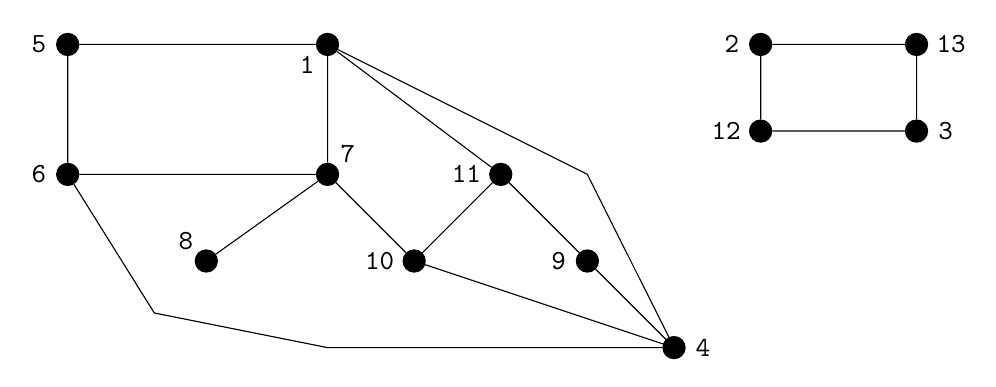
\begin{tikzpicture}[
    scale=1.1,
    label distance=2pt,
    every node/.style={
        font=\ttfamily,
        draw,
        fill=black,
        circle,
        inner sep=0pt,
        minimum size=8pt}]
    \node[label=left:5] (A) at (0,3.5) {};
    \node[label=below left:1] (B) at (3,3.5) {};
    \node[label=above right:7] (C) at (3,2) {};
    \node[label=left:6] (D) at (0,2) {};

    \node[label=above left:8] (E) at (1.6,1) {};

    \node[label=left:10] (F) at (4,1) {};
    \node[label=left:11] (G) at (5,2) {};
    \node[label=left:9] (H) at (6,1) {};
    \node[label=right:4] (I) at (7,0) {};

    \node[label=left:2] (J) at (8,3.5) {};
    \node[label=right:13] (K) at (9.8,3.5) {};
    \node[label=right:3] (L) at (9.8,2.5) {};
    \node[label=left:12] (M) at (8,2.5) {};

    \draw (A) -- (B) -- (C) -- (D) -- (A);
    \draw (C) -- (E);
    \draw (F) -- (G);
    \draw (C) -- (F) -- (I);
    \draw (B) -- (G) -- (H) -- (I);
    \draw (D) -- (1,.4) -- (3,0) -- (I);
    \draw (B) -- (6,2) -- (I);
    \draw (J) -- (K) -- (L) -- (M) -- (J);
\end{tikzpicture}
\newpage

Le tableau ci-dessous donne, pour chaque personne, l'étape à laquelle elle a été placée, ainsi que la maison dans laquelle elle a été placée.

\begin{center}
    \begin{tabular}{| c | c | c |}
        \hline
        personne & maison 1 & maison $-1$\\
        \hline
        1 & 1 & \\
        \hline
        2 & 7 & \\
        \hline
        3 & 9 & \\
        \hline
        4 & & 4 \\
        \hline
        5 & & 2 \\
        \hline
        6 & 3 & \\
        \hline
        7 & & 2 \\
        \hline
        8 & 6 & \\
        \hline
        9 & 5 & \\
        \hline
        10 & 5 & \\
        \hline
        11 & & 2 \\
        \hline
        12 & & 8 \\
        \hline
        13 & & 8 \\
        \hline
    \end{tabular}
\end{center}

\Q
Réflexivité : $a_i,i=1$ pour tout $i$ par convention.\\
Symétrie : s'il existe une suite de personnes de $i$ à $j$ telle que chaque personne est en conflit avec la suivante et la précédente, la même suite dans l'ordre inverse prouve que $a_{i,j}=1$.\\
Transitivité : s'il existe une suite de personnes en conflit de $i$ à $j$ et une autre suite de $j$ à $k$, la concaténation des deux suites donne une suite de personnes en conflit de $i$ à $k$.
\medskip

On a donc une relation d'équivalence. Les classes d'équivalence correspondent à ce que nous avons appelé les \og composantes connexes \fg{}.
\medskip

Clairement, s'il existe une suite de $i_1$ à lui même telle que décrite dans l'énoncé et si $i_1$ est dans la maison 1, alors $i_2$ doit être placé dans la maison $-1$, $i_3$ dans la maison 1, ..., $i_k$ dans la maison $(-1)^{k-1}$, donc $i_{2l+1}$ dans la maison 1 et $i_1=i_{2l+2}$ dans la maison $-1$ : contradiction.
\medskip

Inversement, si la fonction de la question 2 aboutit à la réponse \og partage impossible \fg{}, c'est parce qu'une personne $k$ dans la composante connexe de $i$ se trouve contrainte d'être placée dans les deux maisons à la fois. Il existe donc deux suites de personnes en conflit allant de $i$ à $k$, l'une de longueur paire et l'autre de longueur impaire. La concaténation de la première suite avec la deuxième suite en ordre inverse donne une suite de $i$ à $i$ de longueur impaire.
\medskip

Les différentes classes d'équivalence étant indépendantes les unes des autres, le nombre total de partages sans conflits est le produit du nombre de partages sans conflit pour chaque classe. Ce nombre, pour la classe d'équivalence de $i$ est soit 0 s'il existe une suite impaire de $i$ à $i$, soit 2 sinon : en effet, le premier élément de la classe d'équivalence peut être placé au choix dans la maison 1 ou $-1$, et toutes les autres affectations sont ensuite déterminées par la parité de la longueur de la suite reliant une personne à $i$. Le produit est donc 0 ou $2^N$.

\Q
La première idée consiste à mettre la personne 1 dans la maison 1, son premier ennemi dans la maison 2, et ses ennemis successifs, soit dans la maison 2 s'ils ne sont pas en conflit avec quelqu'un se trouvant déjà dans la maison 2, soit dans la maison 3 sinon. Cela conduirait à une généralisation facile de l'algorithme de la question 2, mais malheureusement cet algorithme ne marche pas : il existe des conflits pour lesquels il ne trouve pas de solution alors qu'il en existe une. Par exemple :
\medskip

$a_{1,2}=a_{1,3}=1$ ;\\
$a_{2,1}=a_{2,3}=a_{2,4}=a_{2,5}=1$,\\
$a_{3,1}=a_{3,2}=a_{3,5}=1$,\\
$a_{4,2}=a_{4,5}=1$,\\
$a_{5,2}=a_{5,3}=a_{5,4}=1$.\\
(Les entrées non définies sont 0). Un algorithme similaire à celui de la question 2 ferait les affectations suivantes :\\
\texttt{maison.(0) <- 1},\\
\texttt{maison.(1) <- 2},\\
\texttt{maison.(2) <- 3},\\
\texttt{maison.(3) <- 1},\\
\texttt{maison.(4)} \og impossible \fg{},\\
alors que les affectations de 1, 2, 3, 4, 5 à 1, 2, 3, 2, 1 satisfont les contraintes.
\medskip

De fait, il n'existe pas de modification astucieuse de l'algorithme qui le rende correct : ce problème, connu sous le nom de coloriage d'un graphe par trois couleurs, est bien connu en informatique théorique pour être difficile. Il n'existe actuellement pas d'algorithme efficace pour le résoudre, c'est-à-dire qui fasse beaucoup mieux que regarder les $3^n$ affectations possibles des personnes dans les maisons.
\medskip

Plus généralement, le problème de coloriage d'un graphe avec le nombre minimum de couleurs, de sorte que deux sommets liés par une arête soient toujours de couleurs différentes, est le problème du nombre chromatique. Un problème célèbre, resté longtemps conjecture, est de démontrer que tout graphe planaire (représentable sur un plan sans que ses arêtes se coupent) a un nombre chromatique au plus égal à 4, ou encore que toute carte planaire peut être coloriée avec au plus 4 couleurs de façon que deux pays ayant une frontière commune soient toujours de couleurs différentes : ceci a finalement été démontré en réduisant l'ensemble de tous les graphes planaires possibles à un nombre fini mais élevé de cas de graphes (environ 1900), qui furent ensuite examinés un par un par ordinateur.
\bigskip

\Fin
